\documentclass[12pt,a4paper]{article}
\usepackage{amsmath}
\usepackage{hyperref}
\usepackage{graphicx}
\usepackage{glossaries}

\title{DocLaTeX Feature Demonstration\thanks{Generated directly from LaTeX.}}
\author{DocLaTeX Project}
\date{2026}

\def\R{\mathbb{R}}
\newcommand{\E}{\mathrm{e}}
\newcommand{\vect}[1]{\mathbf{#1}}
\NewDocumentCommand{\greet}{O{World} m}{Hello #1, #2!}
\newtheorem{theorem}{Theorem}[section]
\newacronym{api}{API}{Application Programming Interface}
\newacronym{cpu}{CPU}{Central Processing Unit}
\newglossaryentry{compiler}{name={compiler},description={A program that translates source code}}
\makeglossaries

\begin{document}
\maketitle
\tableofcontents

\section{Macro expansion and references}\label{sec:macros}
\greet[LaTeX]{user} Vectors such as $\vect{x}\in\R^n$ use expanded macros.
This section is referenced as Section~\ref{sec:macros}, by name \nameref{sec:macros}, and automatically as \autoref{sec:macros}.

The \gls{api} is expanded on first use. Later we write simply \gls{api}; \glspl{cpu} are pluralized.
A \gls{compiler} is also a glossary entry.

\section{Equations}\label{sec:math}
Equation~\eqref{eq:euler} is numbered, while \cref{eq:square} uses a clever reference.
\begin{equation}
  \E = mc^2 \label{eq:euler}
\end{equation}
\begin{align}
  (a+b)^2 &= a^2+2ab+b^2 \label{eq:square}\\
  \int_0^1 x_i^2\,dx &= \frac{1}{3}
\end{align}
An unnumbered display:
\[
  \left(\begin{matrix}a&b\\c&d\end{matrix}\right),\qquad \sqrt{x}\geq 0.
\]

\begin{theorem}\label{thm:sample}
If $x>0$, then $x+x>x$. See \cref{thm:sample}.
\end{theorem}

\section{Lists, tables and figures}
\begin{itemize}
  \item First bullet with \textbf{bold text}.
  \item Second bullet with a footnote\footnote{Footnotes are written to word/footnotes.xml.}.
\end{itemize}
\begin{enumerate}
  \item Numbered item.
  \item Another numbered item.
\end{enumerate}

\begin{table}[ht]
\begin{tabular}{lcr}
\hline
Left & Center & Right\\
\hline
A & B & C\\
1 & 2 & 3\\
\hline
\end{tabular}
\caption{A sample table}\label{tab:sample}
\end{table}
Table~\ref{tab:sample} contains three columns.

\begin{figure}[ht]
\centering

\includegraphics[width=0.25\textwidth]{pixel.png}
\caption{A generated PNG image}\label{fig:pixel}
\end{figure}
Figure~\ref{fig:pixel} is embedded in the DOCX package.

\begin{figure}[ht]
\centering
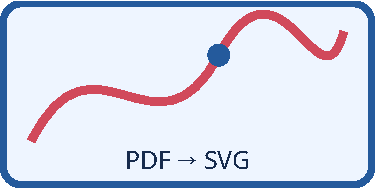
\includegraphics[width=0.45\textwidth]{vector.pdf}
\caption{A PDF figure converted to SVG}\label{fig:vector}
\end{figure}
Figure~\ref{fig:vector} is converted from PDF to SVG before embedding.

\begin{verbatim}
\def\example#1{Value: #1}
verbatim & text $not_math$
\end{verbatim}

\section{Bibliography}
Classic works are cited numerically \cite{knuth1984,lamport1994}. An individual citation is \cite{knuth1984}.
See \href{https://www.latex-project.org/}{the LaTeX project} online.

\printglossaries
\bibliographystyle{plain}
\bibliography{refs}
\end{document}
